\section{Approach}
\label{sec:approach}


In this section, we introduce how to leverage low-level performance information to augment Bayesian Optimization.


\subsection*{Choosing the Low-Level Metrics}

Prior work has shown that low-level performance metrics of workload are a good proxy for predicting performance~\cite{Novakovic2013, Hsu2016, Ousterhout2017, Yadwadkar2017}. For example, the \textit{memory commit size} represents the amount of memory required to handle current workload, and
the \textit{I/O wait time} may indicate a resource bottleneck.
However, in practical settings, we need to analyze multiple metrics for better understanding the key factors that affect performance.
System utilities on Linux, such as \emph{sysstat}, provide a comprehensive set of performance metrics~\cite{sysstat},
which are useful to characterize workloads and identify performance bottlenecks. In this work, we use these low-level metrics to augment BO.
The intuition behind this design choice stems from the fact that the published VM characteristics are inadequate to fully characterize a VM.
In \myfigure{\ref{fig:bottleneck}},
we show that using low-level information helps
identify memory bottleneck of running Logistic Regression.



\begin{figure}[!htbp]
    \centering
    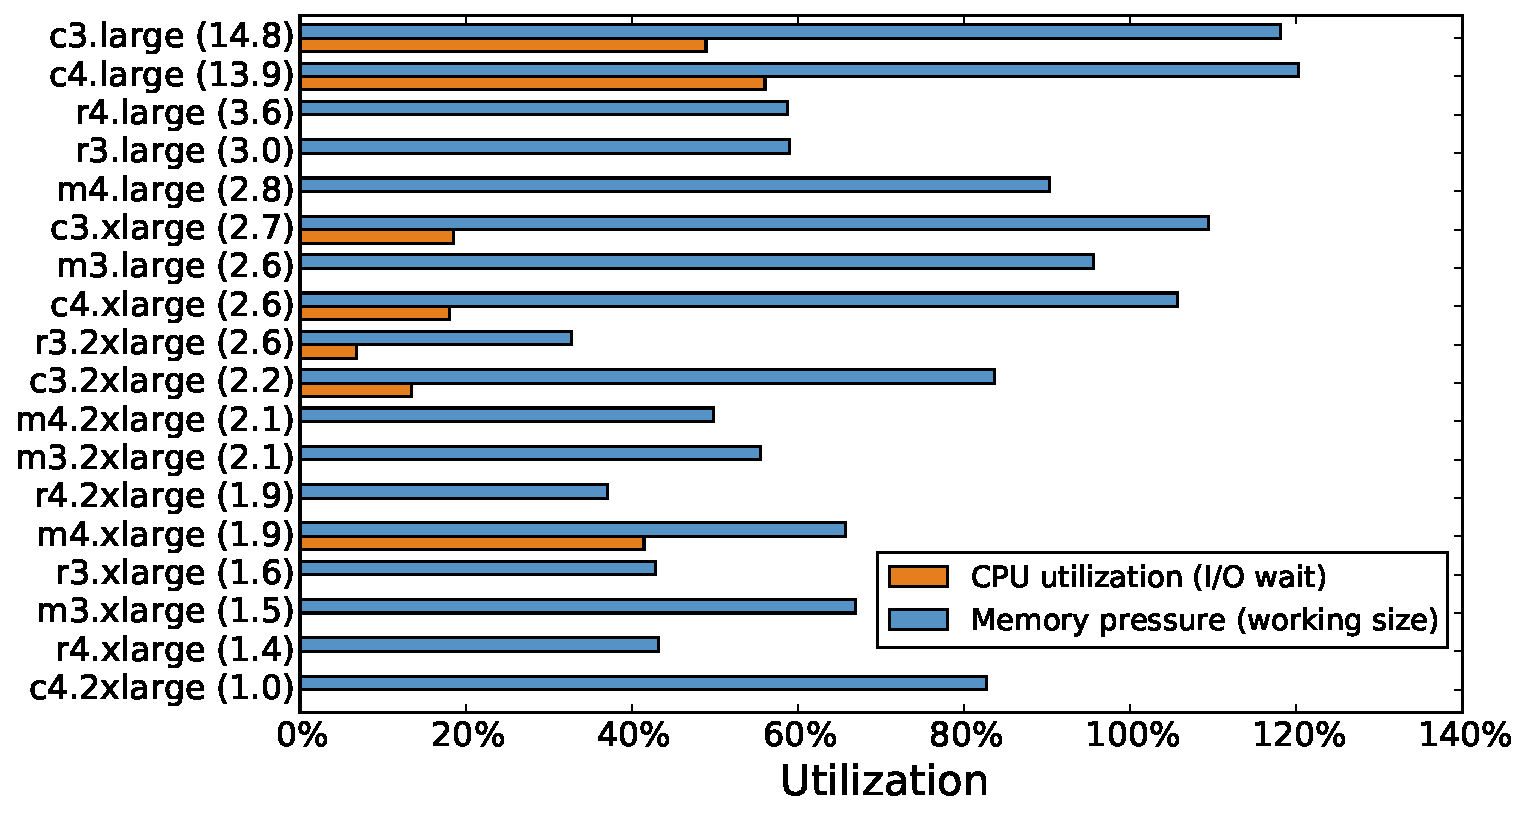
\includegraphics[width=0.8\textwidth]{figures/bottleneck_spark.als.large.pdf}
    \caption{A memory bottleneck is identified by low-level performance information. The horizontal axis represents the resource utilization (\%), and the vertical axis represents the VM types. The numbers in the parenthesis are the normalized execution time where 1.0 represent the best VM type. The memory of a small VM type (c3.large) is not sufficient to run Logistic Regression, which leads to 14.8 times slower than the best VM type (c4.2xlarge). This behavior is captured by memory pressure and CPU utilization. 
}
    \label{fig:bottleneck}
\end{figure}

Since we focus on recurring jobs, we should use metrics that can capture the workload progress and identify resource bottleneck.
The selection of low-level metrics depends heavily on workloads.
If possible, we should use a comprehensive set of metrics.
However, a large number of features can lead to the over-fitting problem in building predictive models.
This is known as the curse of dimensionality~\cite{domingos2012few}.
Automatic feature selection can help address this problem~\cite{guyon2003introduction, Hsu2016} but requires further studies.
In this work, we find the following low-level metrics are effective.


\begin{itemize}
    \item \textbf{Workload progress}: CPU utilization of user space processes and I/O operations, and the number of tasks in the task list.
    \item \textbf{Memory pressure}: \% of commits in memory.
    \item \textbf{I/O pressure}: disk utilization and disk wait time.
\end{itemize}




\iffalse
'cpu.%usr.50',
'cpu.%iowait.50',
'disk.%util.50',
'disk.await.50',
'load.plist-sz.50',
'memory.%commit.50',
\fi

\subsection*{Low-Level Augmented Bayesian Optimization}

Leveraging low-level information in BO requires novel modeling methods because the given workload is yet to be executed on the candidate VM. Our approach, instead, predicts the performance (cost or time) based on the VM characteristics and observed low-level metrics of the VM that is already measured. This is similar to the reasoning technique used in practical settings by experts and the table based models~\cite{Anderson2001}. Experts choose to interpolate or extrapolate the workload performance using not only characteristics of VM but also the low-level performance information.

We make the following design choices to integrate low-level performance information into BO.
Algorithm~\ref{alg:abo} illustrates the Augmented BO.
\begin{algorithm}[htbp]
{
 \SetAlgoLined
 \DontPrintSemicolon
 \DontPrintSemicolon
 \KwIn{$f$, $\mathit{VM}$, $S$, $M$}
 \KwOut{Near-optimal configurations}
 $D$ := Initial sampling ($f$, $\mathit{VM}$) \;

 \For{$k$ in $|\mathit{VM} \notin D|$}{
   $p(y|vm, D, L)$ := FitLowLevelModel(M, D, L) \;
   $vm_k$ := $arg max_{vm \in \mathit{VM}} S(x, p(y|vm, L, D))$ \;
   $y_k, L_k$ := $f(\mathit{vm}_k)$ \;
   $D$ := $D \cup (\mathit{vm}_k, y_k, L_k)$ \;
   \If{meeting stopping criteria}{
        break\;
   }
 }
 \caption{Low-Level Augmented Bayesian Optimization (similar to Algorithm~\ref{alg:smbo})}
 \label{alg:abo}
 }
\end{algorithm}


\begin{itemize}
\item \textbf{Augmented Instance Space}:
Instead of using only VM characteristics ($\mathit{VM}_i$) as an input to the surrogate model,
we also use low-level metrics ($L_i$) collected from running the workload on  ($\mathit{VM}_i$). These constitute the \textit{independent variables}. Similar to Naive BO, the performance of the workload is used as the \textit{dependent variable}.
\textit{Decision to use low-level information allows BO to  make more informed search.}

\item \textbf{Surrogate Model}: Instead of using Gaussian Process as the surrogate model, we choose a tree-based ensemble method Extra-Trees algorithm for building the surrogate model. The tree-based learning method is effective
to capture complex performance behavior
~\cite{Wang2004, Yin2006, Noorshams2013,Hsu2016, Yadwadkar2017}. We choose not to use Gaussian Process in Bayesian Optimization because determining the right kernel function (as discussed in Section~\ref{sec:kernel}) requires careful evaluation, which is not practical for supporting diverse workloads. \textit{This design choice lets us side-step one of the reasons for the fragility of Naive BO}.

\item \textbf{Acquisition Function}: We replace \textit{Expected Improvement} (EI) with \textit{Prediction Delta} as the acquisition function. 
Prediction Delta can be used for selecting a VM type with better performance (shorter execution time or cheaper deployment cost).
Prediction Delta can also be used as a stopping criterion---to terminate the search process if there exists no better VM type. We do not use Expected Improvement as our acquisition function because it is not useful when the kernel function cannot estimate the black-box function. \textit{This design choice for an acquisition function which does not require a suitable kernel function.}

\item \textbf{Surrogate Model Update}: When updating the surrogate model upon a new observation for workload (w) ($\mathit{VM}_{i,w}$, $L_{i,w}$ and $y_{i,w}$), we generate multiple pairs of input ($\mathit{VM}_{j,w}$, $\mathit{VM}_{i,w}$), where $i\neq j$ with
low-level information ($L_{j,w}$), where $j$ represent the source VM---which has been measured and $i$ represents the destination VM---which is yet to be measured.
This surrogate model answers \quotes{what is the predicted performance of $\mathit{VM}_{i,w}$ given the low-level performance information observed on a particular VM ($\mathit{VM}_{j,w}$)}. For example, if we have measured the performance of workload (w) in 3 VMs ($VM_{1,w}, VM_{2,w}, VM_{3,w}$), the number of independent values for which the performance needs to be estimated would be $3 \times (18-3)$.
It should be noted that in order to estimate the performance of a workload in a VM (say $\mathit{VM}_{15,w}$),
we have to consider $\mathit{VM}_{1,w}\rightarrow\mathit{VM}_{15,w}$,  $\mathit{VM}_{2,w}\rightarrow\mathit{VM}_{15,w}$, and $\mathit{VM}_{3,w}\rightarrow\mathit{VM}_{15,w}$.  Since multiple pairs exist, we average the estimated performance. \textit{This design choice helps us update the surrogate model even when the low-level information of destination VM is not available.}

\end{itemize}

\iffalse
\noindent\textbf{Augmented Instance Space}:
Instead of using only VM characteristics ($\mathit{VM}_i$) as an input to the surrogate model,
we also use low-level metrics ($L_i$) collected from running the workload on  ($\mathit{VM}_i$). These constitute the \textit{independent variables}. Similar to Naive BO, the performance of the workload is used as the \textit{dependent variable}.
\textit{Decision to use low-level information allows BO to  make more informed search.}

\noindent\textbf{Surrogate Model}: Instead of using Gaussian Process as the surrogate model, we choose a tree-based ensemble method Extra-Trees algorithm for building the surrogate model. The tree-based learning method is effective
to capture complex performance behavior
~\cite{Wang2004, Yin2006, Noorshams2013,Hsu2016, Yadwadkar2017}. We choose not to use Gaussian Process in Bayesian Optimization because determining the right kernel function (as discussed in Section~\ref{sec:kernel}) requires careful evaluation, which is not practical for supporting diverse workloads. \textit{This design choice lets us side-step one of the reasons for the fragility of Naive BO}.

\noindent\textbf{Acquisition Function}: We replace \textit{Expected Improvement} (EI) with \textit{Prediction Delta} as the acquisition function. 
Prediction Delta can be used for selecting a VM type with better performance (shorter execution time or cheaper deployment cost).
Prediction Delta can also be used as a stopping criterion---to terminate the search process if there exists no better VM type. We do not use Expected Improvement as our acquisition function because it is not useful when the kernel function cannot estimate the black-box function. \textit{This design choice for an acquisition function which does not require a suitable kernel function.}

\noindent\textbf{Surrogate Model Update}: When updating the surrogate model upon a new observation for workload (w) ($\mathit{VM}_{i,w}$, $L_{i,w}$ and $y_{i,w}$), we generate multiple pairs of input ($\mathit{VM}_{j,w}$, $\mathit{VM}_{i,w}$), where $i\neq j$ with
low-level information ($L_{j,w}$), where $j$ represent the source VM---which has been measured and $i$ represents the destination VM---which is yet to be measured.
This surrogate model answers \quotes{what is the predicted performance of $\mathit{VM}_{i,w}$ given the low-level performance information observed on a particular VM ($\mathit{VM}_{j,w}$)}. For example, if we have measured the performance of workload (w) in 3 VMs ($VM_{1,w}, VM_{2,w}, VM_{3,w}$), the number of independent values for which the performance needs to be estimated would be $3 \times (18-3)$.
It should be noted that in order to estimate the performance of a workload in a VM (say $\mathit{VM}_{15,w}$),
we have to consider $\mathit{VM}_{1,w}\rightarrow\mathit{VM}_{15,w}$,  $\mathit{VM}_{2,w}\rightarrow\mathit{VM}_{15,w}$, and $\mathit{VM}_{3,w}\rightarrow\mathit{VM}_{15,w}$.  Since multiple pairs exist, we average the estimated performance. \textit{This design choice helps us update the surrogate model even when the low-level information of destination VM is not available.}
\fi
